% v2-acmtog-sample.tex, dated March 7 2012
% This is a sample file for ACM Transactions on Graphics
%
% Compilation using 'acmtog.cls' - version 1.2 (March 2012), Aptara Inc.
% (c) 2010 Association for Computing Machinery (ACM)
%
% Questions/Suggestions/Feedback should be addressed to => "acmtexsupport@aptaracorp.com".
% Users can also go through the FAQs available on the journal's submission webpage.
%
% Steps to compile: latex, bibtex, latex latex
%
% For tracking purposes => this is v1.2 - March 2012
\documentclass{acmtog} % V1.2
\usepackage[utf8]{inputenc} % Unicode funktioniert unter Windows, Linux und Mac
\usepackage[T1]{fontenc}
% \usepackage{hyperref} % Hyperref funktioniert leider nicht richtig mit bibitem
\usepackage{graphicx}
\usepackage{tikz}
\usepackage[scaled]{helvet}
\usepackage{rotating}
\usepackage[T1]{fontenc}
\usepackage{color}
\usepackage{cclicenses}

%\acmVolume{VV}
%\acmNumber{N}
%\acmYear{YYYY}
%\acmMonth{Month}
%\acmArticleNum{XXX}
%\acmdoi{10.1145/XXXXXXX.YYYYYYY}

\acmVolume{28}
\acmNumber{4}
\acmYear{2009}
\acmMonth{September}
\acmArticleNum{106}
\acmdoi{10.1145/1559755.1559763}

\begin{document}

\markboth{Shahin Imanverdiyev \& Senad Ličina}{Modelling and Conception for Security in Software}

% @shahin: this title is not very good, lets find a better one. our topic is "Modellierung und Entwurf für Security"
\title{Modelling and conception of software in aspect to security} % title

\author{
% 
\includegraphics[width=3.5em]{img/uhh}
\parbox{4.2em}{
\includegraphics[width=3.5em]{img/uhh}}%
\parbox{\textwidth}{
Seminar: Software Architecture \\
Universität Hamburg \\
Shahin Imanverdiyev \& Senad Ličina
}
}

%\category{I.3.7}{Computer Graphics}{Three-Dimensional Graphics and Realism}[Animation]

%\terms{Experimentation, Human Factors}

%\keywords{Face animation, image-based modelling, iris animation, photorealism, physiologically-based modelling}

\maketitle

\begin{bottomstuff}
\today
% Senad Ličina $\bullet$ Seminar: Bio-Inspired Artificial Intelligence $\bullet$ Winter Term 2013/2014
\end{bottomstuff}

\begin{abstract}
%\textcolor{red}{\textbf{DRAFT:} This paper is still under construction!}
\begin{center}
ABSTRACT
\end{center}
% put abstract here.
put Abstract here.
Lorem ipsum dolor sit amet, consectetur adipiscing elit. Donec nec efficitur enim. Mauris leo metus, fermentum dapibus lobortis eu, gravida at libero. Vestibulum eu sem eu sem finibus convallis nec at lectus. Donec finibus dui eget eros bibendum, sit amet pharetra odio rutrum. Etiam sodales suscipit mattis. Sed molestie sagittis rutrum. Vivamus non luctus velit, a venenatis felis. In non sem lacinia, vehicula nisi eget, elementum nibh. Curabitur faucibus est leo, vel placerat lacus dapibus eu. In ut enim a nisl facilisis viverra ut nec tellus.
\end{abstract}

\section{Introduction}

% security is important
Modern society and economy increasingly depend on digital systems.
As attacks against such systems can have devastating results, it is very important to secure such systems in a proper way.
Nowadays the Internet is a heavily used and very important communication medium.
An increasing number of devices are connected to the Internet, which is why it is important to transmit and store sensitive data securely.

% Developing secure systems is difficult
The correct development of secure software is difficult.
There have been numerous successful attacks abusing vulnerabilities of software systems in the past and it can be expected that people will try to detect and abuse such flaws in the future as well.

% System development has to take security aspects into account.
The traditional approach for security assurance has been ``penetrate and patch'', where security is assured by attempting to break into a running system and exploiting well-known vulnerabilities.
Penetrate and patch happens too late in the development process and vulnerabilities will be available and possibly exploited  until they are recognized fixed.
This is why it is important to take security aspects into account in an early stage of the system development.

% Why we should scrap penetrate-and-patch - http://www.cigital.com/papers/download/compass-2.pdf

\section{Requirements}
\label{sec:requirements}

In this section some concepts are explained which are required to understand this paper.
First the key concepts of security are discussed, ...

\subsection{Security Principles}

The CIA Triad is a well-known security model which is based on the three key principles of security: \textbf{confidentiality}, \textbf{integrity} and \textbf{availability}.
It is used to identify problem areas in the security of software systems and requires that its principles are preserved for the system resources.

\begin{description}
	\item[Confidentiality]
		ensures that only authorized users are able to read private or confidential information.
		Access control mechanisms can be used to gain better confidentiality.
	\item[Integrity]
		(in the field of computer security) prevents information from modification or deletion by unauthorized users and ensures that undesired changes can be undone.
	\item[Availability]
		refers to the prevention of unauthorized denial of access to information or resources.
\end{description}

These key principles are often described as incomplete and thus extended by further principles like \textbf{authenticity}, \textbf{accountablility} or \textbf{non-repudiation}.

\begin{description}
	\item[Authenticity] is the assurance that information and resources are valid.
		The validation that all involved parties are truly who they claim to be is important for authenticity.
	\item[Accountablility]
		refers to the property that every security crucial action can be traced back to the responsible
	\item[Non-repudiation]
		assures that the existence of specific actions can not be denied.
\end{description}

\subsection{Unified Modeling Language}

\begin{quote}
	``The Unified Modeling Language (UML) is a general-purpose visual modeling language that is used to specify, visualize, construct, and document the artifacts of a software system.''

	\hfill -- \cite[Chapter 1]{BJR99}
\end{quote}

The Unified Modeling Language (UML) is the prevalent language for the specification of object orientated software systems.
It describes architecture and behavior of software in a graphical manner using various diagram types.

% Although UML is currently available in version 2.x, we will discuss UML 1.5 in this chapter, as the security extension UMLsec (used in Section \ref{sec:umlsec}) is defined for UML 1.5.


\begin{description}
	\item[Use case diagrams] model a systems functionality as percieved by users (or actors).
	Use case diagrams consist of use cases and actors, they can be used to represent interactions between system and user.
	An example for a use case diagram is given with figure \ref{fig:use-case-diagram}.
	The actors (customer, online banking \& banking system) are depicted by stick-figures, the use cases (transfer funds, deposit funds \& withdraw cash) are represented as ovals.
	\begin{figure}[ht]
		\centerline{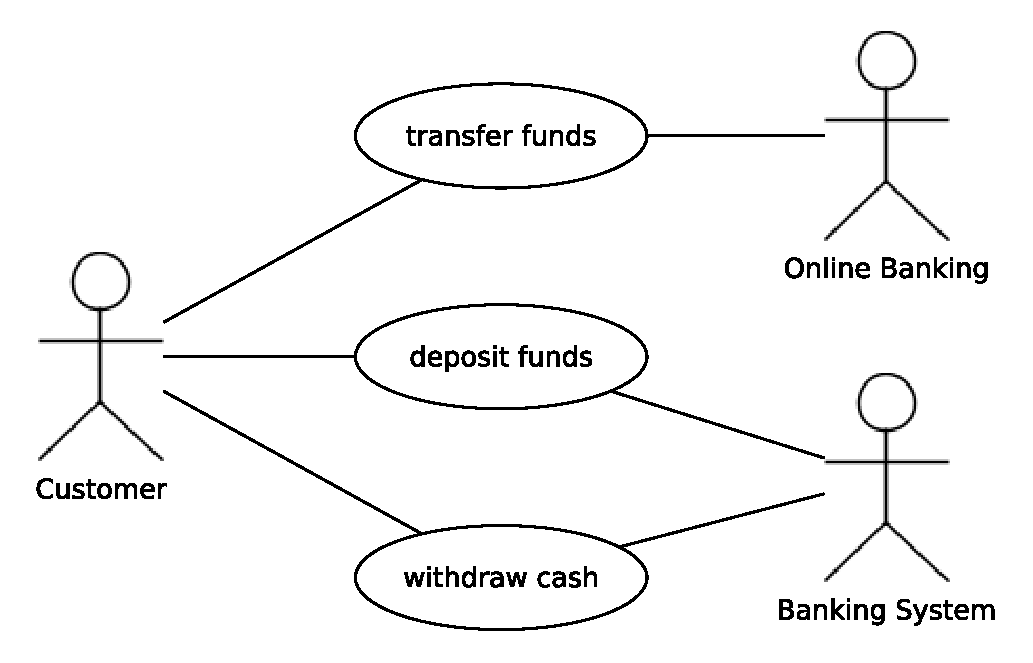
\includegraphics[width=7cm]{img/uml-banking/use-case-diagram}}
		\caption{Example of an use case diagram representing possible interactions between a customer and banking interfaces.}
		\label{fig:use-case-diagram}
	\end{figure}

	\item[Class diagrams] model static concepts within the implementation of an application.
	Classes are drawn as rectangles consisting of three sections for its name, its attributes and its operations.
	Relationships among classes are drawn as paths between them, whereby different arrow types have different meanings.
	Figure \ref{fig:class-diagram} shows a class diagram representing different implementations of the \textit{AccountInterface} and an implementation for the \textit{CustomerInterface}.
	The classes \textit{CheckingAccount} and \textit{SavingsAccount} are inheriting from the class \textit{Account} which is implementing the \textit{AccountInterface}.
	\begin{figure}[ht]
		\centerline{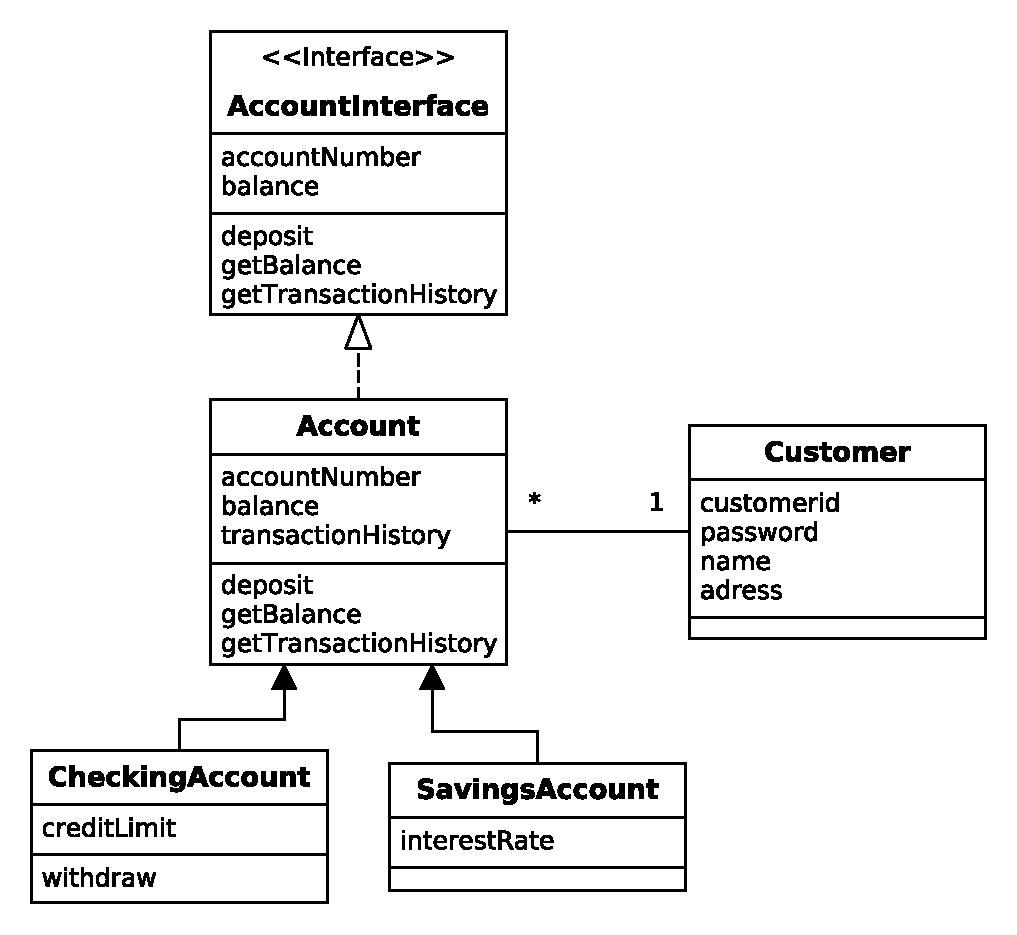
\includegraphics[width=7cm]{img/uml-banking/class-diagram}}
		\caption{A class diagram representing example classes for customer and accounts.}
		\label{fig:class-diagram}
	\end{figure}

	\item[Statechart diagrams] are visual representations of state machines.
	State machines model the sequences of states which an entity can go through.
	States are connected by transitions, which are allowed to have conditions.
	The initial state is depicted by a black dot, the final state as a black dot in a circle.
	Figure \ref{fig:statechart-diagram} shows the states an account object can go through.
	\begin{figure}[ht]
		\centerline{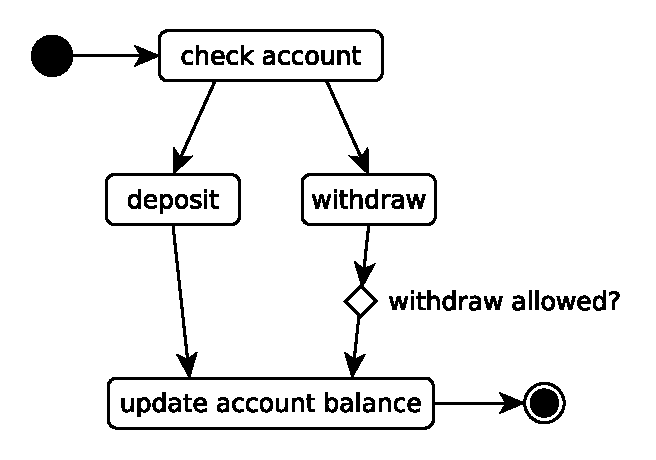
\includegraphics[width=5cm]{img/uml-banking/statechart-diagram}}
		\caption{A statechart diagram depicting the simplified processes cash withdrawal and deposition on an account.}
		\label{fig:statechart-diagram}
	\end{figure}

	\item[Activity diagrams] are a special case of statechart diagrams, used to model processes involving one or more components.
	Activity diagrams make use of synchronization bars to distinguish between sequential and concurrent groups of activities.

	\item[Sequence diagrams] show object interactions by arranging messages in time sequence.
	The vertical lines are lifelines which are representing classifier roles.
	Messages are drawn as arrows between lifelines.
	An example sequence diagram for the scenatio where a customer is withdrawing money at an ATM is given with figure \ref{fig:sequence-diagram}.
	Figure \ref{fig:sequence-diagram} shows an sequence diagram for the example scenario of money withdrawal at an ATM.
	\begin{figure}[ht]
		\centerline{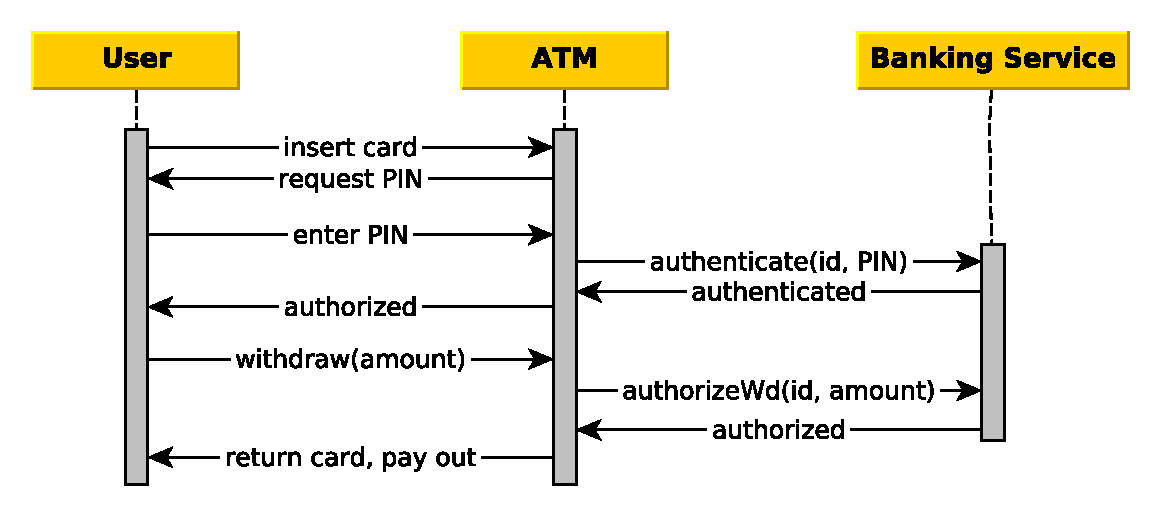
\includegraphics[width=9cm]{img/uml-banking/sequence-diagram}}
		\caption{Money withdrawal at an ATM as a sequence diagram.}
		\label{fig:sequence-diagram}
	\end{figure}

	\item[Deployment diagrams] show networks of conneted nodes, their component instances and objects.
	Nodes are drawn by boxes and may contain components, which are drawn as rectangles with two smaller rectancles on the left side.
	Communication links (on the physical level) are drawn as solid lines connecting nodes, whereas communication dependencies are drawn with broken arrows.
	Communication dependencies can define interfaces and contain class models.
	Figure \ref{fig:deployment-diagram} is a deployment diagram of an example setup for online banking.
	\begin{figure}[ht]
		\centerline{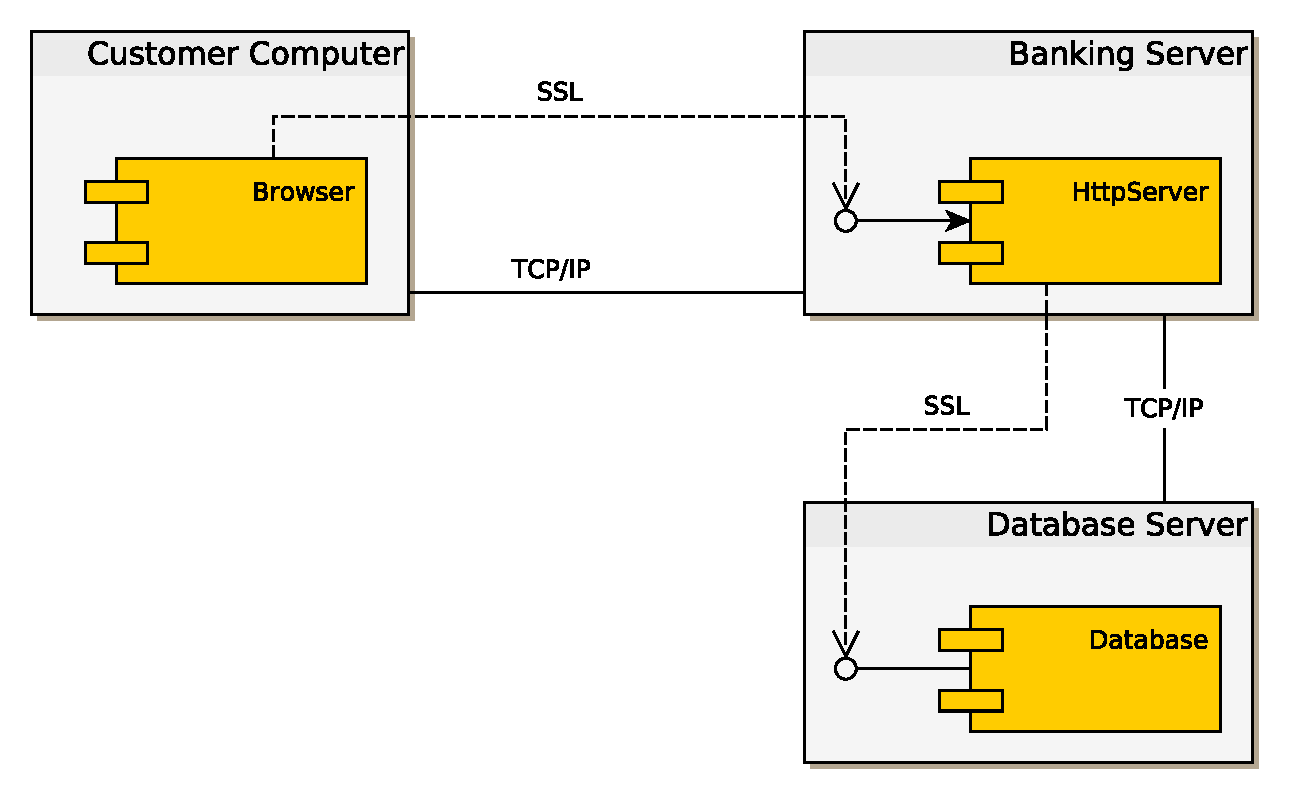
\includegraphics[width=7cm]{img/uml-banking/deployment-diagram}}
		\caption{Online banking infrastructure as a deployment diagram.}
		\label{fig:deployment-diagram}
	\end{figure}
\end{description}

\section{Modeling secure software with UML}
\label{sec:umlsec}

Citation goes like this... \cite{SHRB11}
footnotes \footnote{this is a footnote.} are possible aswell.

Reference to Section \ref{sec:requirements}.

blabla wichtig

intentionally left blank.

\section{Conclusion}
\label{sec:conclusion}

Typical Conclusion.

\section{References}
\renewcommand{\section}[2]{}
\begin{raggedright}%schaltet Blocksatz ab, erzeugt ein stimmigeres Schriftbild im Literaturverzeichnis
\begin{thebibliography}{X}
	\bibitem[BJR99]{BJR99} Grady Booch, Ivar Jacobson, James Rumbaugh: The Unified Modeling Language Reference Manual. Addison-Wesley, Reading (US-MA) 1999.
	\bibitem[JS11]{JS11} Jan Jürjens, Holger Schmidt: UMLsec 4 UML2 - Adopting UMLsec to Support UML2. Technische Universität Dortmund, Dortmund, Germany 2011.
	\bibitem[Jür06]{Jür06} Jan Jürjens: Secure Systems Development with UML. Springer-Verlag, Berlin, Germany 2006.
	\bibitem[SHRB11]{SHRB11} Matthias Straka, Stefan Hauswiesner, Matthias Rüther, Horst Bischof: Skeletal Graph Based Human Pose Estimation in Real-Time. Graz University of Technology, Austria 2011.
\end{thebibliography}
\end{raggedright}

\end{document}
